\documentclass{article}

\usepackage{amsthm}

\newtheoremstyle{mydef}
{\topsep}{\topsep}%
{}{}%
{\bfseries}{}
{\newline}
{%
  \rule{\textwidth}{0.4pt}\\*%
  \thmname{#1}~\thmnumber{#2}\thmnote{\ -\ #3}.\\*[-1.5ex]%
  \rule{\textwidth}{0.4pt}}%

\theoremstyle{mydef}
\newtheorem{definition}{Definition}

\usepackage[hybrid]{markdown}


\title{Notes to Google's Machine Learning Crash Course}
\author{Michael Sendker}
\date{Starting June 27, 2021}

\begin{document}
\begin{markdown}

\maketitle

# Definitions

\begin{definition}[label]
    A label is Y
\end{definition}

\begin{definition}[feature]
    The feature is X
\end{definition}

\begin{definition}[inference]
    running trained model on unlabeled data
\end{definition}

\begin{definition}[regression]
    predicting continuous values (e.g., median house values)
\end{definition}

\begin{definition}[classification]
    predicting discrete values (e.g., hot dog, not a hot dog) also includes
    multi-value classification (e.g., dog, cat, or hamster)
\end{definition}

\begin{definition}[hyperparameters]
    the configuration settings used to tune how the model is trained
\end{definition}

\begin{definition}[empirical risk minimization]
    In supervised learning, a machine learning algorithm builds a model by
    examining many examples and attempting to find a model that minimizes loss;
    this process is called **empirical risk minimization**.
\end{definition}

# Conceptual understanding

Tom helped me understand: all ML is is finding a plane in n-dimensional space
that segregates distinct Ys. The different methods, like Forests, Trees, etc.,
are just different methods of generating functions to distinguish those Ys from
their Xs.

# Reducing Loss

\begin{equation}
    L_2Loss = \sum{(x,y) \in D} (y - prediction(x))^2
\end{equation}

Sometimes useful to average over all examples so divide by $\|D\|$

We use the square of the difference to get a nice concave graph that allows easy
stepping to reduce the loss.


The Derivative of (y-y')² with respect to the weights and biases tells us how
loss changes for a given example.

Repeatedly take small steps in the direction that minimizes loss. These are
called (negative) Gradient Steps. This strategy is called Gradient Descent

\begin{definition}[Gradient Descent]
    The strategy whereby one takes repeated small steps in the direction that
    minimizes loss.
\end{definition}

If your batch is large, testing a lot of steps is extremely expensive, you could
test with one example at a time, or do batches of 10-1000 and average over time.
One example at a time is called **Stocahastic Gradient Descent** and small
batches is **Mini-Batch Gradient Descent**.

I really want to understand the mathy stuff because it's super cool and hard and
I believe I can do it, so, infobox from Google:

## Partial Derivatives

A multivariable function is a function with more than one argument, such as:

\begin{equation}
    f(x,y) = e^{2y}\sin{x}
\end{equation}

The partial derivative of $f$ with respect to $x$, denoted as

\begin{equation}
    \frac{\partial f}{\partial x}
\end{equation}

is the derivative of $f$ as a function of $x$ considered alone. To find
$\frac{\partial f}{\partial x}$ hold $y$ constant and take the derivative of $f$
with respect to $x$.

That seems easy enough. (I'm copying a lot of this verbatim.)

In general, thinking of $y$ as fixed, the partial derivative of $f$ with respect
to $x$ is calculated as follows:

\begin{equation}
    \frac{\partial f}{\partial x}(x,y) = e^{2y}\cos{x}
\end{equation}

and the reverse, $f$ with respect to $y$ holding $x$ fixed:

\begin{equation}
    \frac{\partial f}{\partial y}(x,y) = 2e^{2y}\sin{x}
\end{equation}

It does seem obvious (``intuitive") that the partial derivative of $f$ with
respect to either $x$ or $y$ just tells you how much perturbation in $f$ you get
from either $x$ or $y$.

## Gradients

A **gradient** of a function is the vector of partial derivatives with respect
to all the independent variables, denoted as

\begin{equation}
    \nabla f
\end{equation}

for instance, if

\begin{equation}
    f(x,y) = e^{2y}sin(x)
\end{equation}

then

\begin{equation}
    \nabla f(x,y) =
    \left( \frac{\partial f}{\partial x}(x,y), \frac{\partial f}{\partial y}(x,y) \right) =
    (e^{2y}\cos{x}, 2e^{2y}\sin{x})
\end{equation}

***N.B.*** $\nabla f$ points toward the greatest increase of the function, and
$-\nabla f$ points toward the greatest decrease of the function.

The number of dimensions in the vector is equal to the number of variables in
the formula for $f$; in other words, the vector falls within the domain space of
the function. For instance, the graph of the following function:

\begin{equation}
    f(x,y) = 4 + (x - 2)^2 + 2y^2
\end{equation}

when viewed in three dimenions with $z = f(x,y)$ looks like a valley with a
minimum at (2,0,4):

\begin{figure}[h]
    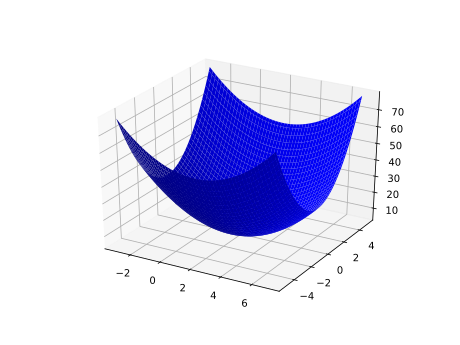
\includegraphics[scale=0.35]{ThreeDimensionalPlot}
    \centering
\end{figure}

# Gradient Descents

A gradient is a vector with a direction and a magnitude. To determine the next
point along the loss function curve, the gradient descent algorithm adds some
fraction of the gradient's magnitude to the starting point. This means we get
diminishing steps.

That's cool, reminds me of Proportional in PID. You halve the distance between
your target and your value. But, like, the gradient is unknown, so your
magnitude is as well, when you're adjusting, and that's the point of the steps.
So how do you know what your Gradient Descent Algorithm (henceforth GDA) should
use as a step?

I guess that's the rub. Or is this something I would just know intuitively from
linear algebra? You know a point, not actually a direction, so it's 50/50 which
way to go on your next iteration.

``The ideal learning rate in one-dimension is $\frac{1}{f(x)''}$.

The ideal learing rate for 2 or more dimensions is is the inverse of the Hessian
(matrix of second partial derivatives)."

What is a Hessian you ask?

\begin{definition}
    In mathematics, the Hessian matrix or Hessian is a square matrix of
    second-order partial derivatives of a scalar-valued function, or scalar
    field. It describes the local curvature of a function of many variables. The
    Hessian matrix was developed in the 19th century by the German mathematician
    Ludwig Otto Hesse and later named after him. Hesse originally used the term
    ``functional determinants".
\end{definition}

Okay, so that's just a matrix of second-order partial derivatives of a
scalar-valued function or scalar field.

I actually get what that is, sort of. I need to learn linalg.

# Starting July 3, 2021

Okay, so I ended up learning linalg, kinda. I watched the 3Blue1Brown videos.

I've got vimtex working with live preview in zathura, much as I don't know that
I like this program.


\end{markdown}

\end{document}
